\documentclass[a4paper,12pt]{article}
\usepackage{jheppub}
\usepackage{taro}

\title{Modern amplitude techniques}

\author[a]{Taro V. Brown}

\affiliation[a]{Department of Physics, UC Davis, One Shields Avenue, Davis, CA 95616, USA }


% e-mail addresses: one for each author, in the same order as the authors
\emailAdd{taro.brown@nbi.ku.dk}


\abstract{Notes on modern amplitude techniques written as part of a research project with Jaroslav Trnka.}

\begin{document} 
\maketitle
\flushbottom
\newpage
\section{Recursion Relations}\label{sec:recursion}
\textit{On-shell recursion is a systematic procedure for relating an amplitude to its
values at singular kinematics. In order to probe these kinematic configurations we define a momentum shift, which is a one-parameter deformation of
the external momenta engineered to sample various kinematic limit}. \\
%
%
A shift of the form
\begin{equation}
p_i\to p_i(z)=p_i+zq_i,~~~~z\in \mathds{C}.
\end{equation}
%
Not all momenta have to be shifted and we restrict the shifted momenta to satisfy momentum conservation as well as being on-shell
%
\begin{equation}
\sum_ip_i(z)=0,~~~~~~p_i(z)^2=0
\end{equation}
%
This implies the following for the shifts $q_i$
%
\begin{equation}
\sum_iq_i=0,~~~~~~q_i^2=q_ip_i=0.
\end{equation}
%
These conditions preserve the kinematics of the corresponding shifted amplitude
%
\begin{equation}
A\to A(z)
\end{equation}
%
We can obtain the original amplitude from the residue
%
\begin{equation}
A(0)=\oint_{z=0}\:\dd z \frac{A(z)}{z}.
\end{equation}
%
One can think of the contour integral as a deltafunction in the point $z=0$.\\
%
Using Cauchy's theorem this can be expressed as minus the sum of all the other residues 
%
\begin{equation}
A(0)=-\sum_I \Res_{z=z_I}\left[\frac{A(z)}{z}\right] +B_\infty,
\end{equation}
%
where $B_{\infty}$ is a boundary term that vanishes when $A(z)\to 0$ for $z\to \infty$. This will be another condition on what variables we shift. \\
%
If we take a subset of momenta $\{p_i\}_{\in I}$ and define the sum over these
%
\begin{equation}
P_I\equiv\sum_{i\in I} p_i,
\end{equation}
%
then we can also defined the shifted momenta $P_I(Z)$
%
\begin{equation}
P_I(z)=\sum_{i\in I} p_i(z)=P_I+zQ_I,~~~~\text{with } Q_I=\sum_{i\in I} q_i
\end{equation}
%
For simplicity we will assume $q_iq_j=0$ leading to $Q_I^2=0$. In this case $P_I(z)^2$ is linear in z
%
\begin{equation}
P_I(z)^2=(P_I+zQ_I)^2=P_I^2+zP_I Q_I=-\frac{P_I^2}{z_I}(z-z_I),
\end{equation}
%
where we have defined $z_I\equiv-\frac{P_I^2}{2P_IQ_I}$.\\
%
\textbf{For some reason} the amplitude should factorize into a product of two lower point on-shell amplitudes when $z=z_I$ and $P_I^2(z)$ goes on-shell
%
\begin{equation}
\lim_{z\to z_I}A(z)=A_L(z_I)\frac{1}{P^2_I(z)}A_R(z_I)=-\frac{z_I}{z-z_I}A_L(z_I)\frac{1}{P^2}A_R(z_I)
\end{equation}
%
Using this to take the residue at $z=z_I$
%
\begin{equation}
=-\Res_{z=z_I}\left[\frac{A(z)}{z}\right]=
\Res_{z=z_I}\left[\frac{z_I}{z(z-z_I)}A_L(z_I)\frac{1}{P_I^2}A_R(z_I)\right]
\end{equation}
%
The residue is found by multiplying by $(z-z_I)$ and setting $z=z_I$. Summing over all residues we find the amplitude
%
\begin{equation}
A(0)=\sum_I A_L(z_I)\frac{1}{P_I^2}A_R(z_I)+B_{\infty}
\end{equation}
%
The boundary contribution $B_\infty$ has no similar general expression in terms of lower-point amplitudes and the simplest way to make it vanish is by requiring  
%
\begin{equation}
A(z)\to 0,~~~~~\text{for } z\to \infty
\end{equation}
%
If this holds then 
%
\begin{equation}
A=\sum_I A_L(z_I)\frac{1}{P_I^2}A_R(z_I)=\sum_{\text{Diagrams }I} 	\raisebox{-.5\height}{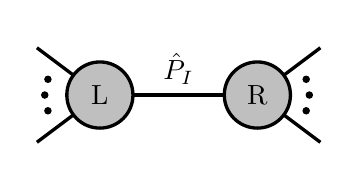
\begin{tikzpicture}[xscale=2,yscale=2]
\draw [style= very thick] (0.6,0.3) -- (1,0) node[at start, above] {};
\draw [style= very thick] (0.6,-0.3) -- (1,0) node[at start, below] {};
\draw [style= very thick] (1,0) -- (2,0) node[midway, above] {$\hat P_{I}$};
\draw [style= very thick] (2,0) -- (2.4,0.3) node[at end, above] {};
\draw [fill=black] (0.65,0) circle [radius=0.02];
\draw [fill=black] (0.67,0.1) circle [radius=0.02];
\draw [fill=black] (0.67,-0.1) circle [radius=0.02];
\draw [fill=black] (2.33,0) circle [radius=0.02];
\draw [fill=black] (2.31,0.1) circle [radius=0.02];
\draw [fill=black] (2.31,-0.1) circle [radius=0.02];
\draw [style= very thick] (2,0) -- (2.4,-0.3) node[at end, below] {};
\draw [style=very thick,fill=lightgray] (1,0) circle [radius=0.21] node[] {L};
\draw [style=very thick,fill=lightgray] (2,0) circle [radius=0.21] node[] {R};
\end{tikzpicture}}
\end{equation}
%
%
%
\subsection{BCFW-recursion}
%
A particular recursion technique used often is called BCFW recursion. In four dimensions this can be implemented in the spinor-helicity basis. Denoting the shifted variables by a hat, the shifts that we will employ are
\begin{equation}
\begin{aligned}
|\hat i]=|i]+z|j],~~~~|\hat j]=|j],~~~~|\hat i \rangle = | i \rangle,~~~~|\hat j \rangle =|i\rangle-z|j\rangle
\end{aligned}
\end{equation}

%
\subsection{Example of BCFW-recursion}
%
As an example, let us calculate the amplitude $A_5(1_g^+,2_g^-,3_g^+,4_g^-,5_g^-)$
Since we are dealing with an $\overline{\text{MHV}}$ amplitude we can immediately read of the good shift since the shifts
\begin{align}
|1]\to|\hat{1}]&=|1]+z|5]\\
|5\rangle\to|\hat{5}\rangle&=|5\rangle-z|1\rangle
\end{align}
will shift the amplitude by
\[
A_{5}(1^+,2^-,3^+,4^-,5^-)=\frac{[13]^4}{[12][23][34][45][51]}\to \frac{\expval{([13]+z[53])^4}}{([12]+z[52])[23][34][45]}\sim z^3
\]
While the shifts
\begin{align}
|5]\to|\hat{5}]&=|5]+z|1]\\
|1\rangle\to|\hat{1}\rangle&=|1\rangle-z|5\rangle
\end{align}
will shift the amplitude by
\[
A_{5}(1^+,2^-,3^+,4^-,5^-)=\frac{[13]}{[12][23][34][45][51]}\to \frac{[13]^4}{[12][23][34]([45]+z[41])([51]\underbrace{+z[11]}_{0})}\sim \frac{1}{z}
\]
Now since we want $A\to 0$ for $z\to \infty$ the \textit{good shift} is the second one, meaning [5] $|1\rangle$ which corresponds to a $[-,+\rangle$ shift in Elvangs notation.
%
We could have seen the good shifts by little group scaling of the amplitude since leg one has little group weight 1 and so will the amplitude under a shift will scale like z if we shift the square brackets
 The corresponding diagrams are

\begin{figure}[H]
	\centering
	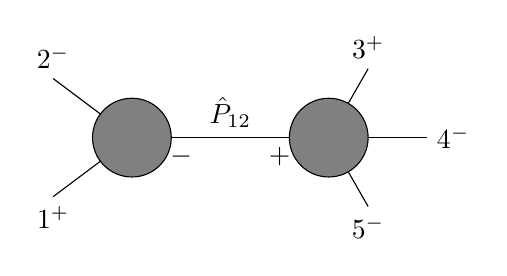
\begin{tikzpicture}[xscale=2.5,yscale=2.5]
	\draw (0.6,0.3) -- (1,0) node[at start, above] {$2^-$};
	\draw (0.6,-0.3) -- (1,0) node[at start, below] {$1^+$};
	\draw (1,0) -- (2,0) node[midway, above] {$\hat P_{12}$} node[near end, below] {$+$} node[near start, below] {$-$};
	\draw (2,0) -- (2.5,0) node[at end, right] {$4^-$};
	\draw (2,0) -- (2.2,0.35) node[at end, above] {$3^+$};
	\draw (2,0) -- (2.2,-0.35) node[at end, below] {$5^-$};
	\draw [fill=gray] (1,0) circle [radius=0.2];
	\draw [fill=gray] (2,0) circle [radius=0.2];
	\end{tikzpicture}
\end{figure}
\begin{figure}[H]
	\centering
	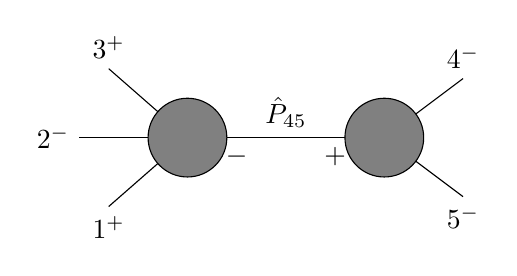
\begin{tikzpicture}[xscale=2.5,yscale=2.5]
	\draw (0.6,0.35) -- (1,0) node[at start, above] {$3^+$};
	\draw (0.6,-0.35) -- (1,0) node[at start, below] {$1^+$};
	\draw (0.45,0) -- (1,0) node[at start, left] {$2^-$};
	\draw (1,0) -- (2,0) node[midway, above] {$\hat P_{45}$} node[near end, below] {$+$} node[near start, below] {$-$};
	\draw (2,0) -- (2.4,0.3) node[at end, above] {$4^-$};
	\draw (2,0) -- (2.4,-0.3) node[at end, below] {$5^-$};
	\draw [fill=gray] (1,0) circle [radius=0.2];
	\draw [fill=gray] (2,0) circle [radius=0.2];
	\end{tikzpicture}
\end{figure}
Looking at the first diagram we see that it contains a 3-point MHV amplitude
\begin{equation}
A_3(1^+,2^-,-\hat P_{12}^-)=\frac{\expval{2\hat P_{12}}^3}{\expval{\hat 1 2}\expval{\hat P_{12}\hat 1}}
\end{equation}
Since we impose that the propagating momentum is on shell we see that
\[
0=\hat{P}_{12}=\expval{\hat 1 2}[\hat 1 2]=\expval{\hat 1 2}[1 2]
\]
So the only way to impose on shell conditions is by setting $\expval{\hat 1 2}=0$ similarly one can show that the numerator vanishes and we must have 
\[
A_3(1^+,2^-,-\hat P_{12}^-)=0
\]
which means the first diagram doesn't contribute. For the second diagram we also have a 3-point MHV amplitude, but in this case the shift is in |5] so the sub-diagram isn't zero.

We can then proceed to calculate the second diagram explicitly
\begin{align*}
A_{5}(1^+,2^-,3^+,4^-,5^-)&=A_3(\hat{P}_{45}^+,4^-,\hat 5^-)\frac{1}{P_{45}^2}A_4(\hat 1,^+,2^-,3^+,-\hat P_{45}^-)\\
&=\frac{\expval{4\hat 5}^3}{\expval{\hat P_{45}4}\expval{\hat 5\hat P_{45}}}\frac{1}{\expval{45}[45]}\frac{[\hat 13]^4}{[\hat 12][23][3\hat P_{45}][\hat P_{45}\hat 1]}
\end{align*}
Since the shift is in $[5,1\rangle$ we can remove the hat on all but the $P$'s: 
\begin{align*}
A_{5}(1^+,2^-,3^+,4^-,5^-)
&=\frac{\expval{4 5}^3}{\expval{\hat P_{45}4}\expval{5\hat P_{45}}}\frac{1}{\expval{45}[45]}\frac{[13]^4}{[12][23][3\hat P_{45}][\hat P_{45} 1]}\\
&=\frac{\expval{4 5}^3}{\expval{\hat P_{45}4}\expval{5\hat P_{45}}}\frac{1}{\expval{45}[45]}\frac{[13]^4}{[12][23][3\hat P_{45}][\hat P_{45} 1]}
\end{align*}
We can the rewrite the $\hat P$ terms in the following way:
\begin{align*}
\expval{\hat P_{45}4}[\hat P_{45}1]&=-\expval{4\hat P_{45}}[\hat P_{45}1]=\langle 4|\hat P_{45}|1]=\langle 4|4+\hat{5}|1]=\langle 4|\hat{5}|1]=-\expval{4\hat 5}[\hat 5 1]=-\expval{45}[5 1]\\
\expval{5\hat P_{45}}[3\hat P_{45}]&=-\expval{5\hat P_{45}}[\hat P_{45}3]=\langle 5|\hat P_{45}|3]=\langle 5|4+\hat{5}|4]=\langle 5|4|3]+\langle 5|\hat 5|3]\\
&=-\expval{54}[ 4 3]-\expval{5\hat 5}[ \hat 5 3]=-\expval{54}[ 4 3]=-\expval{45}[34]
\end{align*}
where we in the first terms have used the fact that $|\hat 5\rangle=|5\rangle$ and $[\hat 5 1]=[51]+z[11]=[51]$, while in the second term using $\expval{5\hat 5}=\expval{5 5}=0$. Inserting this into the amplitude we get
\begin{align*}
A_{5}(1^+,2^-,3^+,4^-,5^-)
&=\frac{[13]^4\expval{45}^3}{[12][23][45]\expval{45}^3[51][34]}\\
&=\frac{[13]^4}{[12][23][34][45][51]}
\end{align*}
which is the expected result.
\subsection*{Part b}
The soft-limit factorization for tree amplitudes is that for $k_s\to 0$ we can write an n-point amplitude as
\begin{equation}
A_n^{\text{tree}}(1,2,\dots,a,s^\pm,b,\dots,n)=\mathcal{S}(a,s^\pm,b)\times A_{n-1}^{\text{tree}}(1,2,\dots,a,b,\dots,n)
\end{equation}
where
\begin{equation}
\mathcal{S}(a,s^+,b)=\frac{\expval{ab}}{\expval{as}\expval{sb}},\qquad \mathcal{S}(a,s^-,b)=-\frac{[ab]}{[as][sb]}
\end{equation}
Here this gets us
\begin{align*}
A_{5}(1^+,2^-,3^+,4^-,5^-)=-\frac{[41]}{[45][51]}\times\frac{[13]^4}{[12][23][34][41]}
\end{align*}
which is a valid factorization of the full result.

In the collinear limit for leg 1 and 2 we have the two momenta $k_1$ and $k_2$ that become parallel with intermediate momentum $k_P$. The spinors also have the following relations
\begin{align*}
&\lambda_a\simeq\sqrt{z}\lambda_P,\qquad \lambda_b\simeq \sqrt{1-z}\lambda_P\\
&\tilde\lambda_{\dot a}\simeq\sqrt{z}\tilde\lambda_P,\qquad \tilde\lambda_{\dot b}\simeq \sqrt{1-z}\tilde\lambda_P
\end{align*}
taking the amplitude we calculated in part a and shifting it in this limit gives
\[
A_5(1^+,2^-,3^+,4^-,5^-)\to \frac{z^2}{\sqrt{z(1-z)}[12]}\frac{[P3]^4}{[P3][34][45][5P]}
\]
which is the result we expected from Dixon:
\begin{equation}
A_{n}^{\text{tree}}(\dots,a^{\lambda_a},b^{\lambda_b},\dots)\to \sum_{\lambda_p=\pm}\text{Split}_{-\lambda_P}(a^{\lambda_a},b^{\lambda_b};z)A^{\text{tree}}_{n-1}(\dots,P^{\lambda_P},\dots)
\end{equation}
where
\begin{equation}
\text{Split}_{-}(a^+,b^-)=\frac{z^2}{\sqrt{z(1-z)}[ab]}
\end{equation}
%
\newpage
\begin{thebibliography}{99}

%\cite{Bjerrum-Bohr:2013bxa}
\bibitem{Bjerrum-Bohr:2013bxa}
N.~E.~J.~Bjerrum-Bohr, J.~F.~Donoghue and P.~Vanhove,
``On-shell Techniques and Universal Results in Quantum Gravity,''
JHEP \textbf{02} (2014), 111
doi:10.1007/JHEP02(2014)111
[arXiv:1309.0804 [hep-th]].
%83 citations counted in INSPIRE as of 21 Aug 2020

%\fi
\end{thebibliography}
\end{document}

